\subsection{Visualization}
To demonstrate the potential applications of Synopsis, we created two visualizations. Our first visualization generated a climate chart by issuing statistical queries to retrieve high, low, and mean temperature values as well as precipitation information for a given spatial region. Climate charts are often used to provide a quick overview of the weather for a location; Figure~\ref{fig:climate} summarizes the temperature and precipitation in Snowmass Village, Colorado during 2014. While a standard approach for producing these visualizations over voluminous atmospheric data would likely involve several MapReduce computations, our sketchlets make all the necessary information readily available through queries, avoiding distributed computations altogether. Furthermore, retrieving the data for this evaluation consumed considerably less time (1.5 ms) than drawing the image on the client side (127.1 ms).

\begin{figure}[h]
    \centerline{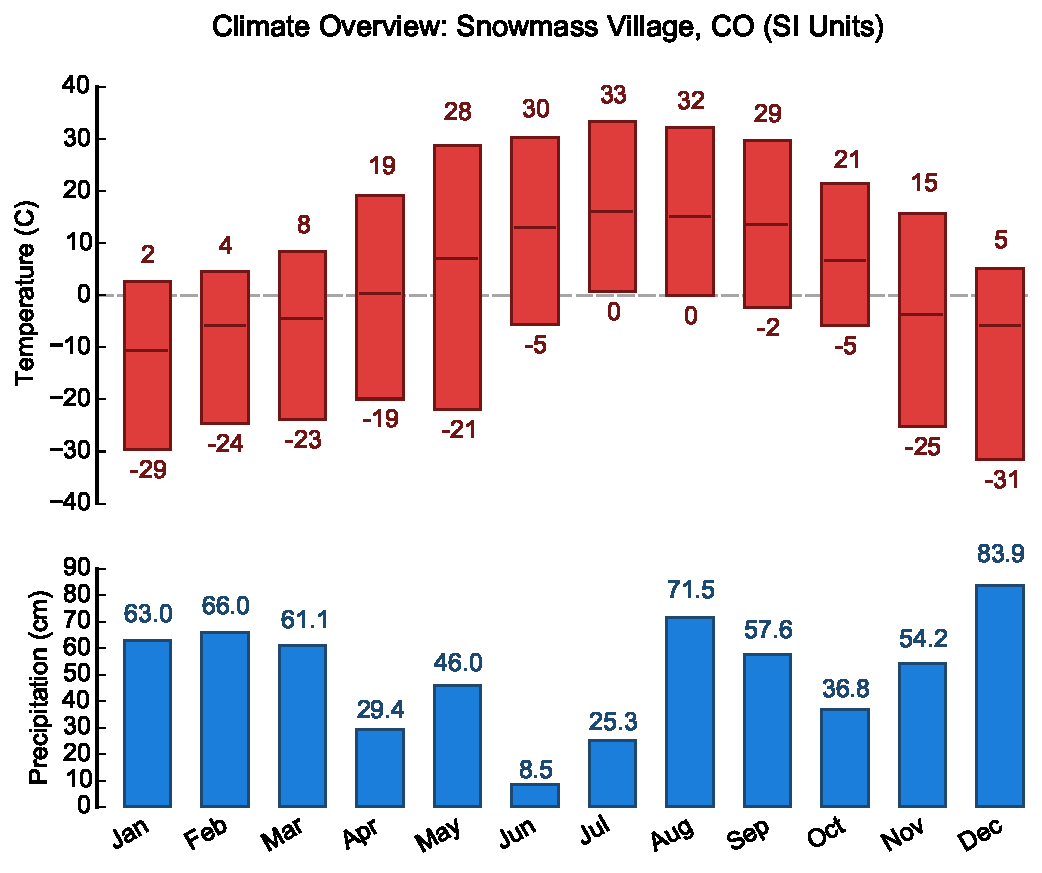
\includegraphics[width=\linewidth]{figures/climate-snowmass.pdf}}
    \caption{A climate chart generated with our statistical query functionality.}
    \label{fig:climate}
\end{figure}

Our second visualization issued queries to retrieve cloud cover information for the entirety of North America. To reduce processing load on the client side, we specified minimum visibility thresholds to eliminate data points that would not be visible in the final output figure. After retrieving this information, we executed a second query that located all areas that exhibited high correlations between cloud cover and precipitation. Figure~\ref{fig:global-contour} illustrates the results of this process for data in July of 2014; cloud cover is represented by white contours with varying opacity, while blue contours describe the correlation between cloud cover and precipitation (darker blues, such as those seen in the top-center of the globe, represent a stronger correlation). Due to the large scope of this visualization (retrieving all data points for a given month across all spatial regions), retrieval took approximately 2.82 seconds, with graphics rendering consuming an additional 1.51 seconds at the client application.

\begin{figure}[h]
    \centerline{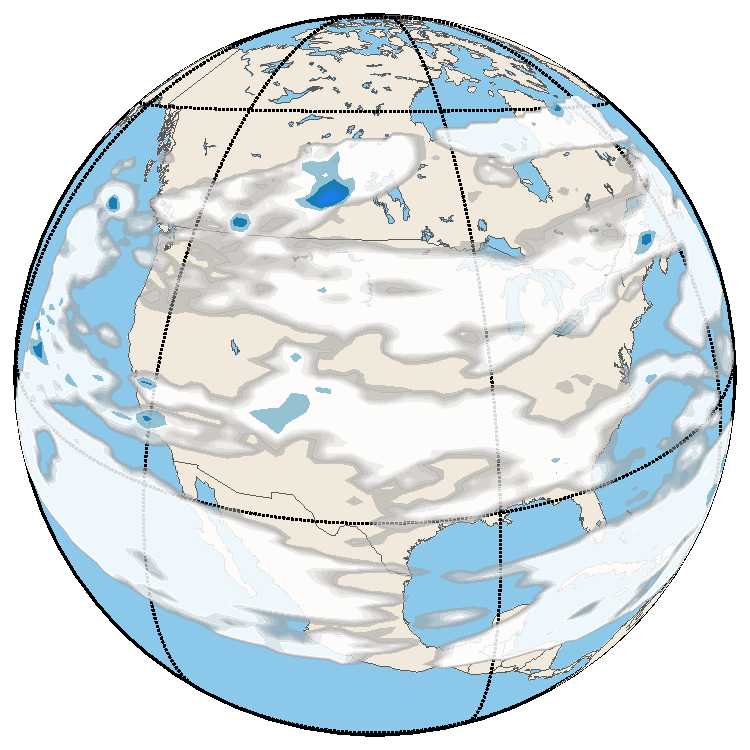
\includegraphics[width=2.85in]{figures/globe.pdf}}
    \caption{Global contour visualization}
    \label{fig:global-contour}
\end{figure}

\subsection{Use with Analytic Engines}
Synthetic data queries in \textsc{Synopsis} can be used to generate representative datasets that require less space while still providing high accuracy.  
Such datasets can be used efficiently with analytic engines such as Apache Spark \cite{zaharia2010spark} and TensorFlow \cite{tensorflow}.  
We used Spark to train regression models based on the Random Forest ensemble method to predict temperatures (in Kelvin) using surface visibility, humidity and precipitation in the southeast United States during the months of May--August, 2011--2014.
These models were generated using the original full-resolution data as well as synthetic data sets that were sized at 10\% and 20\% of the original data.
The accuracy of these models was measured using a test dataset extracted from actual observations (30\% of the overall dataset size).
All five datasets were staged on HDFS and loaded into Spark to train the ensemble models.

We evaluated the efficacy of our approach based on the on-disk and in-memory storage requirements, data loading time, training time and the accuracy of the model.
Our observations are summarized in Table~\ref{tab:spark-rf}.
The accuracy of the models generated based on synthetic data is comparable to those of models generated using actual data, while requiring less space, training and loading times.
For instance, our 10\% synthetic dataset produces a model with similar accuracy incurring 54\% less training time while reducing space requirements by 90\%. Additionally, based on the number of RDD partitions used, the synthetic datasets require substantially less computing resources.
%
\begin{table*}[ht!]
    \renewcommand{\arraystretch}{1.2}
    \caption{Comparing Random Forest based regression models generated by Spark MLlib using synthetic vs. real data \vspace{-1em}}
    \label{tab:spark-rf}
    \begin{center}
        \begin{tabularx}{\textwidth}{|X|c|c|c|c|c|c|c|c|}
            \hline
            \multirow{2}{*}{Dataset} & \multirow{2}{*}{Size (GB)} & \multirow{2}{*}{RDD Partitions} & \multicolumn{2}{c|}{\cellcolor[gray]{0.7}Data Loading Time (s)} &\multicolumn{2}{c|}{\cellcolor[gray]{0.7}Model Training Time (s)} & \multicolumn{2}{c|}{\cellcolor[gray]{0.7}Accuracy - RMSE (K)}\\
            \cline{4-9}
             & & & \cellcolor[gray]{0.9}Mean & \cellcolor[gray]{0.9}Std. Dev.  &  \cellcolor[gray]{0.9}Mean & \cellcolor[gray]{0.9}Std. Dev. &  \cellcolor[gray]{0.9}Mean & \cellcolor[gray]{0.9}Std. Dev. \\
            \hline
            Original & 25.350 & 208 & 28.035 & 2.249 & 506.493 & 9.500 & 5.981 & 0.027 \\
            \hline
            Original - 10\% Sample & 2.535 & 21 & 5.136 & 0.909 & 205.627 & 5.798 & 5.960  & 0.049 \\
            \hline
            Original - 20\% Sample & 5.069 & 41 & 6.102 & 1.607 & 216.857 & 7.994 & 5.994 & 0.026 \\
            \hline
            Synthetic - 10\% & 2.549 & 21 & 5.097 & 0.912 & 231.221 & 13.459 & 5.951 & 0.027 \\
            \hline
            Synthetic - 20\% & 5.098 & 41 & 6.208 & 0.637 & 235.018 & 16.148 & 5.981 & 0.051 \\
            \hline
        \end{tabularx}
    \end{center}
    \vspace{-1em}
\end{table*}
%
%TODO discussion on why RMSE is actually better for the smaller datasets


